\documentclass[tikz]{standalone}
\begin{document}
\begin{tikzpicture}
    \node[anchor=south west,inner sep=0] at (0,0) {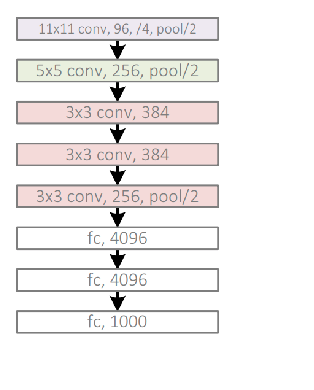
\includegraphics[width=0.6\textwidth]{figs/alex.png}};
    \draw[red,ultra thick,rounded corners] (0.,1.) rectangle (6,2.2);
 
    \fill[white] (2.55,1.4) rectangle (3.8,1.8);
\node[text=black] (c) at (2.6,1.6) {5};
   \node[text=red] (d) at (-1.5,1.5) {New layer};
   \draw[black,ultra thick] (0,2.3) edge[<->] node[left] {freeze} (0,8.5);
\end{tikzpicture}
\end{document}